% Created 2021-03-28 Sun 13:09
% Intended LaTeX compiler: pdflatex
\documentclass[12pt]{article}
\usepackage[utf8]{inputenc}
\usepackage[T1]{fontenc}
\usepackage{graphicx}
\usepackage{grffile}
\usepackage{longtable}
\usepackage{wrapfig}
\usepackage{rotating}
\usepackage[normalem]{ulem}
\usepackage{amsmath}
\usepackage{textcomp}
\usepackage{amssymb}
\usepackage{capt-of}
\usepackage{hyperref}
\usepackage[natbib=true]{biblatex} \DeclareFieldFormat{apacase}{#1} \addbibresource{~/data/Dev/UdacityMLEngineer/capstone/bibliography/references.bib} \usepackage{array} \usepackage{graphicx} \graphicspath{ {./results/eda/}{./results/} }
\usepackage{parskip}
\author{Andrew Pope}
\date{\today}
\title{Capstone Project - Machine Learning Engineer Nanodegree}
\hypersetup{
 pdfauthor={Andrew Pope},
 pdftitle={Capstone Project - Machine Learning Engineer Nanodegree},
 pdfkeywords={},
 pdfsubject={},
 pdfcreator={Emacs 27.1 (Org mode 9.4.4)}, 
 pdflang={English}}
\begin{document}

\maketitle

\section*{Definition}
\label{sec:orgdc365d1}

\subsection*{Project Overview}
\label{sec:org2c3a54a}
Toxicity is a common problem in online forums and comment sections. Many people have had the experience of opening the comment section of an article only to be met with insults, obscenity, and hatred. Extensive human moderation is one solution, but at large scale it's quite costly, and it can be a harrowing task citep:verge-2019-facebook-moderation. The ability to augment human moderation with machine learning models to filter out the worst and most obvious toxic comments is critical.

In this project, I created a classifier to identify several types of toxicity in online comments, including threats, obscenity, insults, and identity-based hate. This problem was originally posed in the Toxic Comment Classification Kaggle competition citep:kaggle-toxic-comments. 
\subsection*{Problem Statement}
\label{sec:org0a10041}
The solution is to create a machine learning model that takes in the text of a comment and outputs a score for each of the toxicity labels, denoting the probability that the comment falls under one of those categories of toxicity. The scores would be used to flag comments for manual inspection by human moderators.
\subsection*{Metrics}
\label{sec:orgb3c0f42}
The main evaluation metric will be the mean label-wise ROC AUC:
\begin{equation}
\frac{1}{L} \sum_{l=1}^{L} AUC_{l}
\end{equation}
where L is the number of labels (in this case 6). ROC AUC is a good metric for this problem because it's indifferent to the classification threshold and it can handle cases where the label is very sparse, like this.

Additionally, the ROC AUC, precision and recall for each individual label will be analyzed as certain labels will be easier to identify than others. Accuracy will be reported, but it's not a good metric when there's so much class imbalance.
\section*{Analysis}
\label{sec:org6a3b183}

\subsection*{Data Exploration}
\label{sec:org02b715e}
The Kaggle dataset contains two files: the training data with 159,571 examples, and the test data with 153,164. In the test data, there are 89,186 examples without labels--these are Kaggle's final test set--and 63,978 with labels. Since this project wasn't intended to be uploaded to Kaggle, I threw out the unlabeled examples in the test set and combined the remaining examples with the training set for a final size of 223,549 examples across my training, validation, and test sets.

Table \ref{table:1} shows some summary data on each label. There are quite a few examples for the toxic, threat, and insult labels, but very few for threat. In all, 22.2\% of examples have at least one positive label.

\begin{center}
\begin{table}
\begin{tabular}{| m{5em} | m{1.5cm} | m{1.5cm} | m{1.5cm} | m{1.5cm} | m{1.5cm} | m{1.5cm} |}
\hline
\multicolumn{7}{|c|}{Label} \\
\hline
& Toxic & Severe Toxic & Obscene & Threat & Insult & Identity Hate \\
\hline
\% of Examples & 9.57\% & 0.878\% & 5.43\% & 0.308\% & 5.06\% & 0.947\% \\
\hline
\# of Examples & 21,348 & 1,962 & 12,140 & 689 & 11,304 & 2,117 \\
\hline
\end{tabular}
\caption{Summary data for labels}
\label{table:1}
\end{table}
\end{center}

These comments have some problematic characteristics. There is quite a bit of punctuation in some that will have to be stripped out, and many comments have an IP address stamped at the end which will also have to be removed.

\subsection*{Exploratory Visualization}
\label{sec:orgbc972b1}

Figure \ref{fig:label-corr} shows the correlations between labels. The highest correlations are between each pair of toxic, obscene, and insult. Threat is not highly correlated with any other label because it's so sparse.

\begin{figure}
\centering
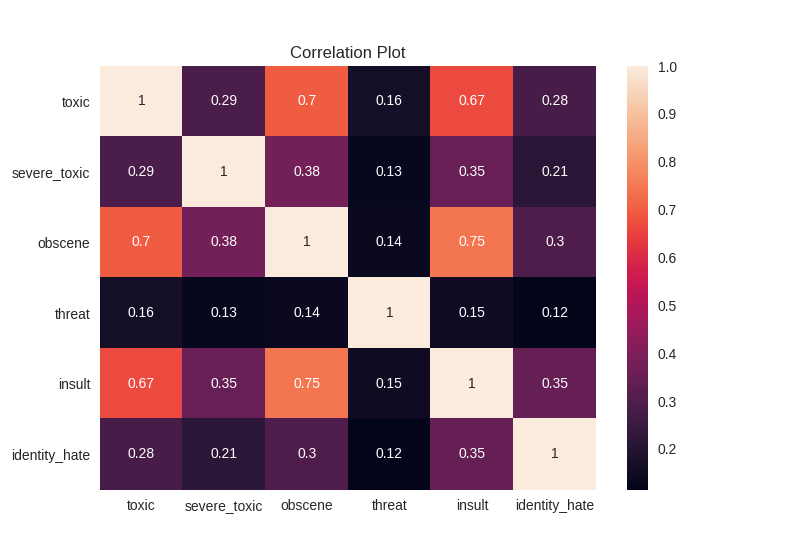
\includegraphics[width=\textwidth]{label_correlations}
\caption{Pearson correlation coefficients for each pair of labels}
\label{fig:label-corr}
\end{figure}

Investigating the comment texts themselves, most comments are fairly short. Figure \ref{fig:character-dist} shows the distribution of character lengths: 79.0\% of examples are less than 500 characters in length, but there is a long tail of longer comments up to 5,000 characters.

\begin{figure}
\centering
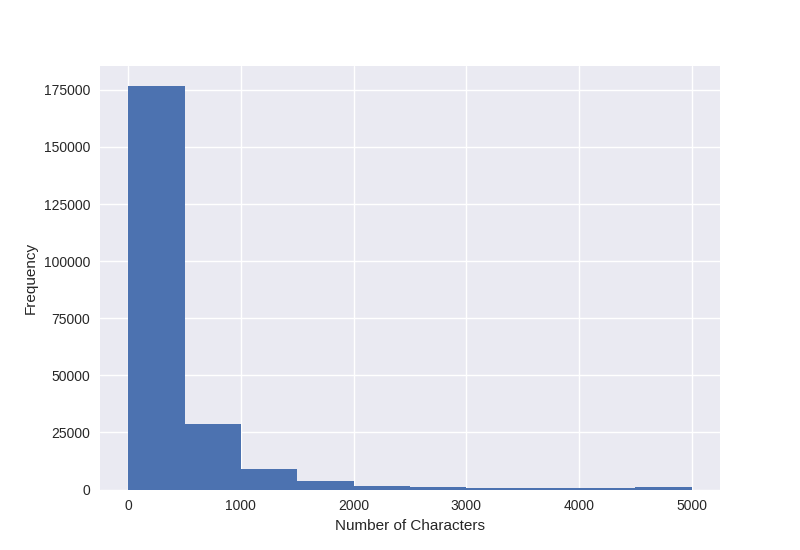
\includegraphics[width=\textwidth]{character_lengths}
\caption{Distribution of the number of characters per example}
\label{fig:character-dist}
\end{figure}

Figure \ref{fig:word-dist} shows a similar pattern for word counts: most comments are fairly short--54.0\% are less than 40 words--while there is also a long tail of comments up to 2,000 words.
\begin{figure}
\centering
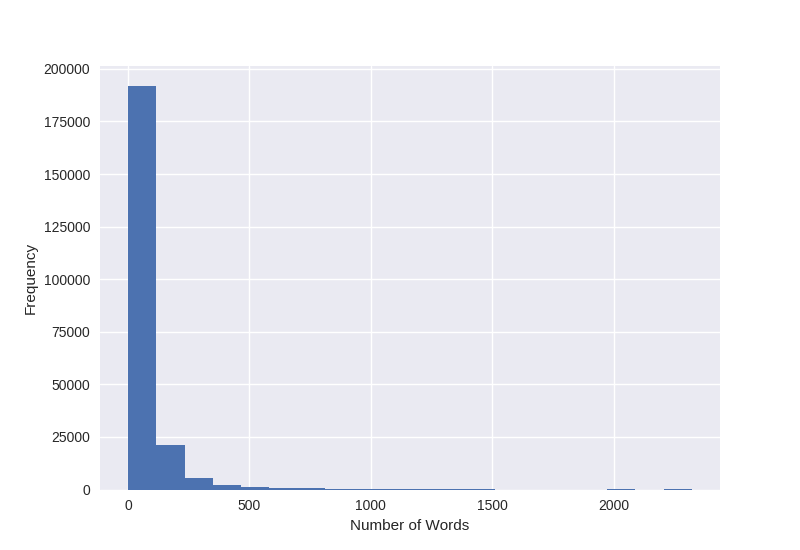
\includegraphics[width=\textwidth]{word_counts}
\caption{Distribution of the number of words per example}
\label{fig:word-dist}
\end{figure}

\subsection*{Algorithms and Techniques}
\label{sec:org11b7dde}
The classifier I used is a multiayer network consisting of an embedding layer, one or many LSTM layers, one or many fully connected layers with ReLU activations (these depend on the hyperparameters of the run), and finally a 6-node layer with sigmoid activation, one for each class label. LSTMs should be much more performant on this problem than non-recurrent approaches because context is very important in identifying some of these classes. For example, identifying identity hate will require the model to understand the context in which an identity is being invoked: a comment saying "I'm <X identity> and therefore I hate <something>" is not identity hate, whereas "I hate <X identity>" is. A simple bag of words approach would not do a very good job of telling one from the other. On the other hand, obscenity is probably easy to identify with just a bag of words: either there's an obscene word in the comment or there isn't.

\subsection*{Benchmark}
\label{sec:org6391af7}
Jigsaw/Conversation AI, the company that sponsored the Kaggle competition, have their own model citep:jigsaw-model-project, a convolutional neural network trained with GloVe word embeddings. Their model achieved an ROC AUC of 0.96857. It's not clear to me whether this is on the exact same dataset as used in this project, but it's still a good benchmark nonetheless.

\section*{Methodology}
\label{sec:org99d4458}

\subsection*{Data Preprocessing}
\label{sec:org454c425}
The preprocessing is done in prep.ipynb and works as follows:
\begin{enumerate}
\item Each comment is cleaned by removing anything that looks like an IP address (see the note Data Exploration), converting all whitespace into spaces, removing punctuation, and lowercasing the text.
\item Each comment is tokenized using nkltk's word\textsubscript{tokenize} function, stop words--any word that exists in nltk's english stop words dictionary--are removed, misspellings of edit distance <= 2 are removed by using SymSpell's dictionary (this step was added later; see note in Refinement), and finally each token is lemmatized using nltk's WordNetLemmatizer
\item A dictionary of the 10,000 most common words from the previous step is created.
\item Each comment is encoded using the dictionary. Comments are padded or truncated to the max length of 500 words (before preprocessing this would handle 98.7\% of comments in the dataset), and then each word is converted into an integer representation based on the dictionary. If a word is not included in the dictionary, it is replaced with a "missing in vocab" token. The final vocabulary size after this step is 10,002: 10,000 words plus the padding token and the missing token. Finally, the original length of the comment is prepended to the encodings and the labels are prepended to that to make one single array: [label1, label2, \ldots{}, label6, comment length, word1, word2, \ldots{}, word500]
\item The results are split into training, validation, and test sets. First, 10\% is reserved for the test set, then 20\% of the remaining (18\% of the total) is reserved for the validation set and the rest (72\%) is used for training. To make sure there are enough examples of each class in each set, these splits are stratified based on a class label (this step was added later; see note in Refinement). For simplicity, that class label is calculated as the maximum positive label for each comment (1-6). Ideally it would be stratified so that each combiniation of labels is considered its own class, but there ends up not being enough examples for that method to work.
\end{enumerate}

\subsection*{Implementation}
\label{sec:orgbb8ef0b}
For each iteration, the training and evaluation happens in test.ipynb. The process is as follows:
\begin{enumerate}
\item Upload the dictionary and training and validation datasets to S3 so they're available to the SageMaker estimator.
\item Create an estimator and load both the training and validation datasets into memory. For the training set, samples are weighted inversely to the frequency of their class (this step was added later; see note in Refinement and see Data Preprocessing step \#5 for the class calculation). The model is trained using the Adam optimizer and binary cross entropy loss with a batch size of 512. During training, the loss function is printed for the training set after each epoch, along with a set of metrics calculated on the validation set: accuracy, precision, recall and ROC AUC. For each of those metrics, each of the individual class-wise metrics are printed along with the average across classes. As mentioned above, the average ROC AUC is the primary metric.
\item After training is completed, I looked at the log outputs to see the final ROC AUC, and whether it continued to increase during training or if it started overfitting.
\item The last run to create the final model used hyperparameter optimization. The hyperparameters tested were:
\begin{itemize}
\item embedding dimension of 32 or 64
\item number of LSTM layers between 1 and 4
\item number of hidden layers and their dimensions: [100], [100, 64], [100, 64, 32], [100, 64, 32, 16]
\end{itemize}
I configured SageMaker to read the average ROC AUC printed to the log and use that as the objective measure and early stopping metric. In all, 20 models were trained before settling on the best model.
\end{enumerate}

\subsection*{Refinement}
\label{sec:org7d811ea}
The initial run I tried didn't use stratified sampling to create the training/validation/test sets, didn't try to correct misspelled words, used a 32-dimension embedding layer, 1 LSTM layer, and 1 100-dimension fully connected layer. When I tried to run the validation metrics, I ran into a problem: there weren't any samples with the threat label in the validation set! So I needed to update the train/val/test splitting to stratify on the class label. With 6 independent labels, that was a bit tricky. Ideally, I wanted to stratify on each possible combination of labels (2\textsuperscript{6} combinations) to make sure each data set has a representative sample, but unfortunately there aren't enough samples in each combination for that to work. So instead I went with a simpler but cruder method: an example is labeled with its max positive class (1-6 for each of the labels, or 0 if all labels are 0). I re-ran the train/val/test split using that class to stratify, and I also added a step to the training script to weight examples based on that class: inversely proportional to the class's prevalence in the training set.

The second run used the same hyperparameters as the first run, with the only difference being those class weights. The results are shown in table \ref{table:2}. The ROC AUC looks decent, but it hides the real problem: precision and recall are quite low. To get a better understanding of what's happening, I tried looking at a sample of false negatives for the Identity Hate label, which was one of the lowest performing. In the examples I saw (which were horrible and I hope to never read again), many of the racial slurs and other important features were misspelled, so I decided to add a step to the preprocessing to replace misspelled words with their dictionary word. This is acheived using SymSpell's lookup function to replace any word within a max edit distance of 2.

\begin{center}
\begin{table}
\begin{tabular}{| m{5em} | m{1.5cm} | m{1.5cm} | m{1.5cm} | m{1.5cm} | m{1.5cm} | m{1.5cm} | m{1.5cm} |}
\hline
\multicolumn{2}{|c}{} & \multicolumn{6}{c|}{Label} \\
\hline
& \textbf{Average} & Toxic & Severe Toxic & Obscene & Threat & Insult & Identity Hate \\
\hline
\textbf{ROC AUC} & 0.872 & 0.903 & 0.875 & 0.920 & 0.857 & 0.917 & 0.761 \\
\hline
\textbf{Accuracy} & 96.9\% & 92.5\% & 98.9\% & 96.2\% & 99.7\% & 95.5\% & 98.9\% \\
\hline
\textbf{Precision} & 49.2\% & 60.6\% & 38.3\% & 65.2\% & 41.7\% & 55.6\% & 33.8\% \\
\hline
\textbf{Recall} & 40.0\% & 62.8\% & 26.0\% & 64.1\% & 11.5\% & 54.5\% & 20.7\% \\
\hline
\end{tabular}
\caption{Validation set metrics for run 2}
\label{table:2}
\end{table}
\end{center}


\section*{Results}
\label{sec:orgb2a955a}

\subsection*{Model Evaluation and Validation}
\label{sec:org17f2faf}
\begin{figure}
\centering
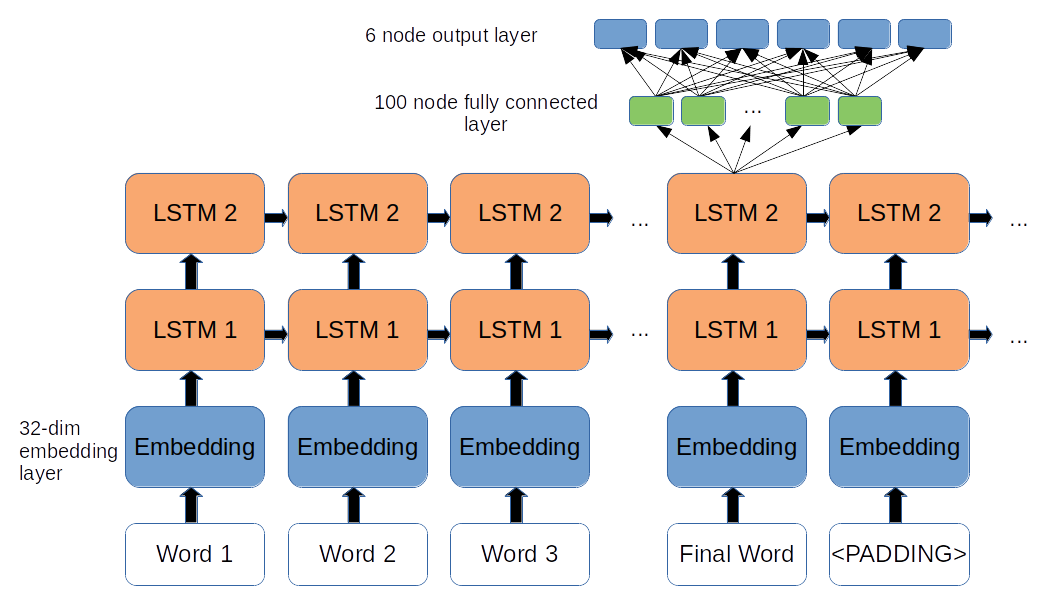
\includegraphics[width=\textwidth]{network}
\caption{Final network structure}
\label{fig:network}
\end{figure}

After hyperparameter tuning, the best model looks like figure \ref{fig:network}. There's a 32-dimension embedding layer, 2 LSTM layers, a 100-dimension fully connected layer, and finally a 6-dimension output layer with a sigmoid activation function.

\begin{center}
\begin{table}
\begin{tabular}{| m{5em} | m{1.5cm} | m{1.5cm} | m{1.5cm} | m{1.5cm} | m{1.5cm} | m{1.5cm} | m{1.5cm} |}
\hline
\multicolumn{2}{|c}{} & \multicolumn{6}{c|}{Label} \\
\hline
& \textbf{Average} & Toxic & Severe Toxic & Obscene & Threat & Insult & Identity Hate \\
\hline
\textbf{ROC AUC} & 0.970 & 0.960 & 0.982 & 0.981 & 0.964 & 0.972 & 0.962 \\
\hline
\textbf{Accuracy} & 96.8\% & 89.6\% & 99.1\% & 97.1\% & 99.7\% & 96.6\% & 99.0\% \\
\hline
\textbf{Precision} & 46.4\% & 48.5\% & 42.3\% & 70.2\% & 0.00\% & 67.7\% & 49.7\% \\
\hline
\textbf{Recall} & 49.3\% & 88.4\% & 26.0\% & 79.8\% & 0.00\% & 66.8\% & 34.7\% \\
\hline
\end{tabular}
\caption{Test set metrics for the final model}
\label{table:3}
\end{table}
\end{center}

\begin{figure}
\centering
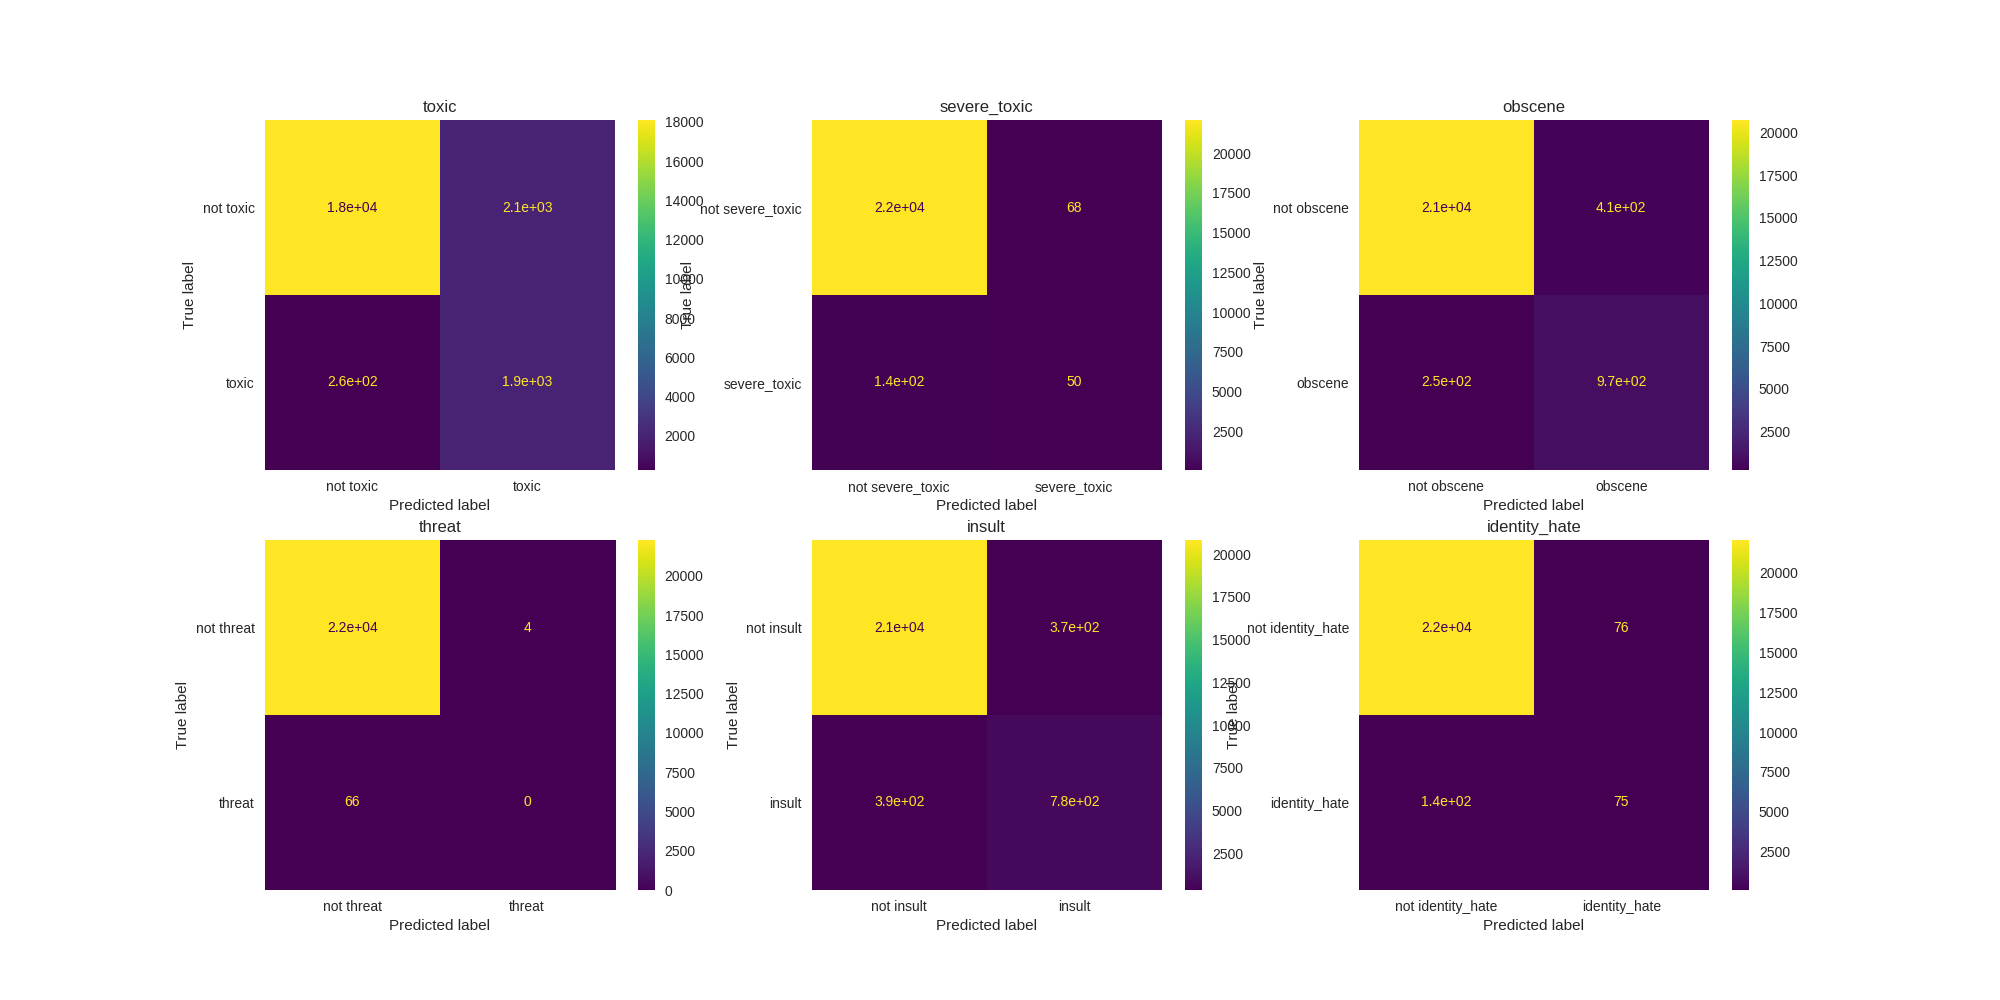
\includegraphics[width=\textwidth]{confusion_matrix}
\caption{Confusion matrices for each label, evaluated on the final test set}
\label{fig:confusion-matrix}
\end{figure}

\begin{figure}
\centering
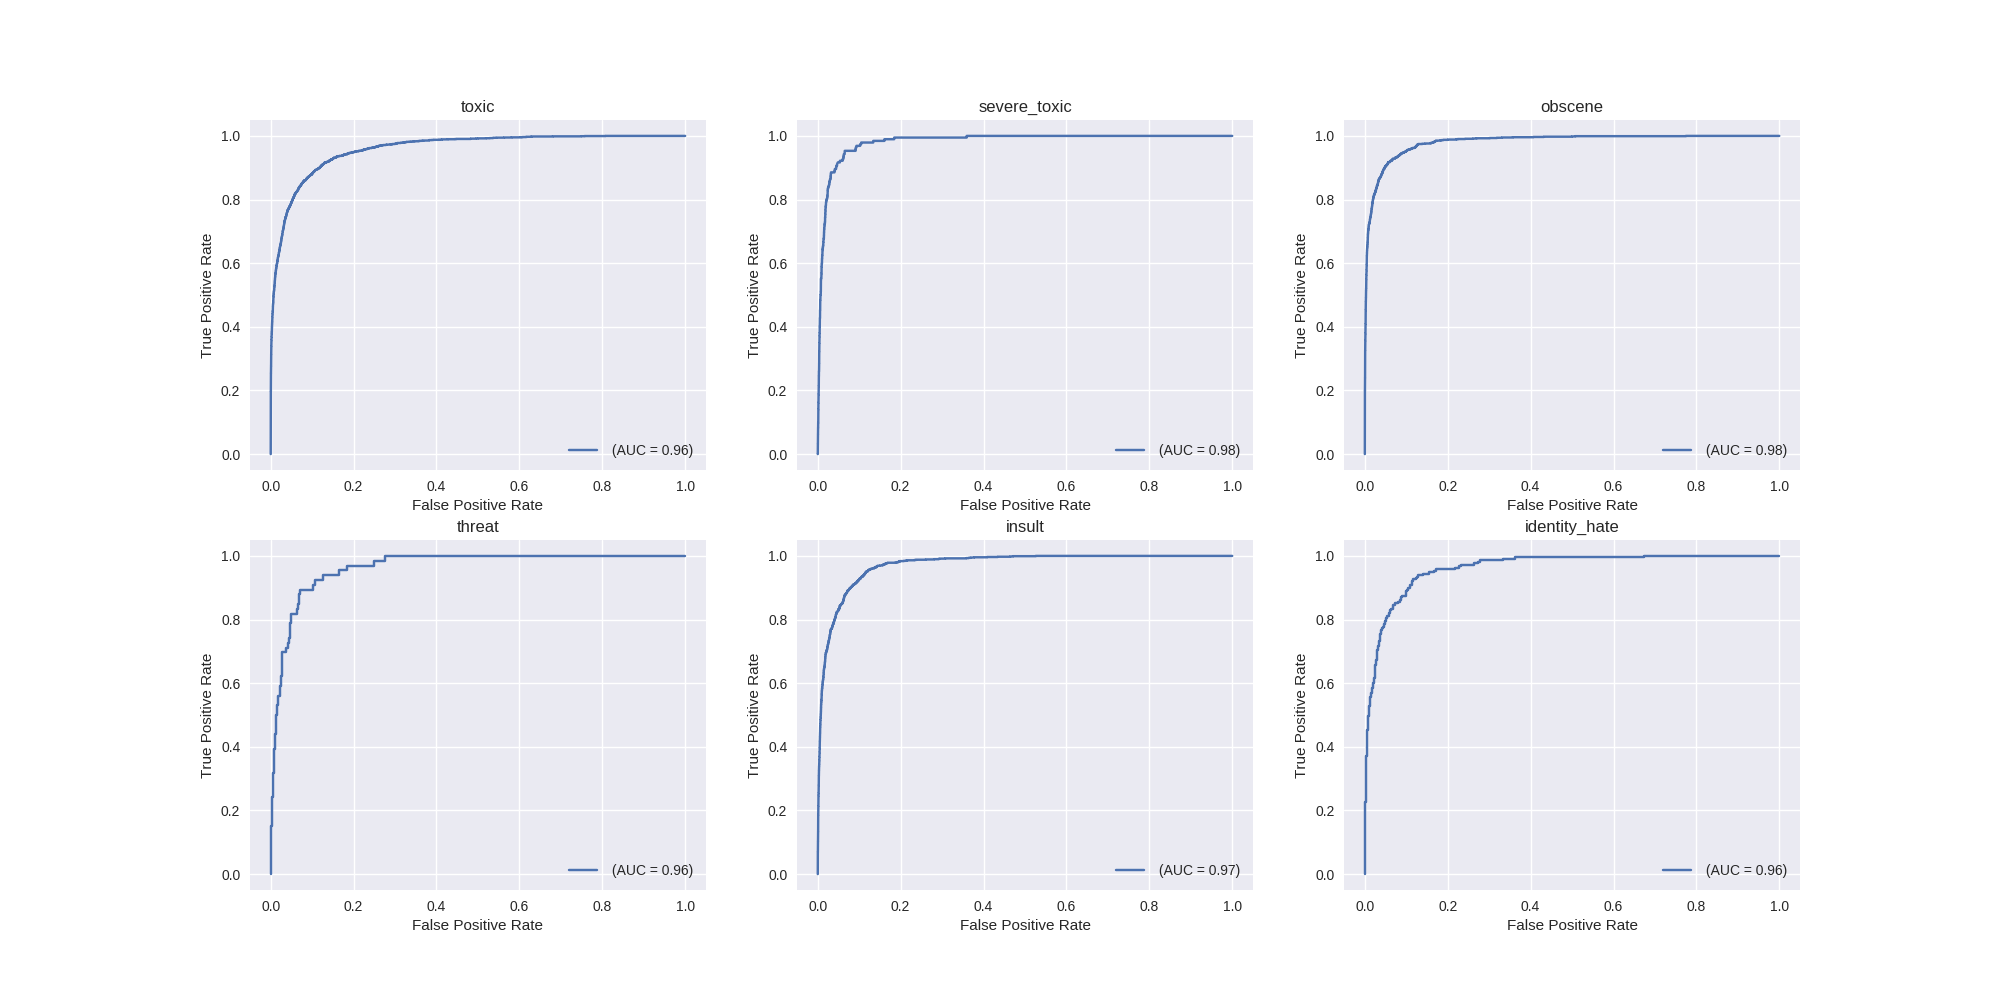
\includegraphics[width=\textwidth]{roc_curve}
\caption{ROC curves for each label, evaluated on the final test set}
\label{fig:roc-curve}
\end{figure}


This model had a 0.9717 ROC AUC on the validation set. After finishing training, I evaluated the model on the test set in final\textsubscript{eval.ipynb}. The summary metrics are shown in table \ref{table:3}. The confusion matrices for each class are in figure \ref{fig:confusion-matrix}. The ROC curves for each class are in figure \ref{fig:roc-curve}.

By label, the performance varies pretty significantly. The easier labels to predict seem to be toxic, obscene, and insult. That makes some sense: toxic is the label for which we have the most data, and obscenities and insults could be captured pretty well just by looking at the individual words in the comment without much context. It's also interesting to note that these are the 3 classes that have higher correlations between them.

Severe toxic and identity hate are more difficult for the model to identify. Looking through examples, I myself had a hard time telling toxic comments from severe toxic ones, so it makes sense to me that the model didn't pick up on the patter. Finally, threat didn't work at all, at least with the default threshold: no comments were correctly classified as a threat in the test set.\footnote{As a side note, I intended to show some examples of comments that were correctly and incorrectly predicted for each class, but I decided against it because they're so awful to read. I investigated examples in the last cell of train.ipynb, and there's one example left in the output.}
\subsection*{Justification}
\label{sec:org2edc244}
The final ROC AUC for this model is 0.970, a bit higher than the benchmark model of 0.96857. Given that these models are probably running on slightly different datasets, I would say these results are comparable but not obviously better.
\section*{Conclusion}
\label{sec:orgfe1c477}
While ROC AUC is a good metric for model comparison, it doesn't capture what the behavior of the model would be in the real world. For that, we should look at recall and precision. Unfortunately the picture is not so rosey. Some types of toxicity, like toxicity with 89\% recall or obscenity with 82\% recall, are relatively easy to identify, but others are much more difficult, like threats with only 4\% recall. In the real world, this model would need to be augmented with some sort of functionality for users to manually flag toxic comments that were missed. Likewise, the precision of this model is too low to be acceptable on its own. No one wants their bengign comment deleted because of a false positive. In the real world, comments flagged by this model would have to be sent to a human moderator before being removed.
\section*{References}
\label{sec:org0d7e2c6}
\printbibliography[heading=none]
\end{document}
